\graphicspath{
    {figures_and_references/urban_surface_detection/}
    {figures_and_references/EELISA_conference/}
    {figures_and_references/footprints_paper/}
}

% \selectlanguage{english}
\renewcommand{\chapternametext}{Chapter \thechapter . Use case: Remote sensing attributes, building height, construction year, and roof material in the 3 pilot regions}
\renewcommand{\shortchapternametext}{Chapter \thechapter . Use case: Height, year and roof material}

\begin{refsection}

\chapter{\chapternametext}
\

\renewcommand{\headingtextL}{}
\renewcommand{\headingtextR}{\shortchapternametext}
\begingroup
 \flushbottom
 \setlength{\parskip}{0pt plus 1fil}%
 \localtableofcontents 
\endgroup

\begingroup
 \flushbottom
 \setlength{\parskip}{0pt plus 1fil}%
 \locallistoffigures
\endgroup


\newpage

\setcounter{section}{0} 

\FloatBarrier

\renewcommand{\sectionnametext}{Building height}
\renewcommand{\headingtextR}{\thesection. \sectionnametext}
\section{\sectionnametext}

All manual surveys conducted in the three pilot regions recorded the number of floors of the buildings. However, the research group had access to a drone and the possibility of conducting surveys and photogrammetric data collection only in Santo Domingo, Dominican Republic. Therefore, the height estimation methodology could be tested solely in this region. Assuming an average height of 3 meters per floor, the survey results were compared with those obtained from the drone flight (fig. \ref{fig:abs_error}), and all cases with height discrepancies were reviewed using Street View imagery. Instances of errors in the survey or differences in interpretation were found. Some buildings have protrusions or sections that are one or two stories higher than the rest of the structure, so depending on the viewpoint chosen during the survey, different results may be obtained. All discrepancies found could be explained as human errors in the survey. The mean absolute error comparing drone and survey heights was 3,2 meters. 

However, errors can still occur if the road network is not accurately positioned and a point is mistakenly taken from a structure. These errors are minimized through the use of Gaussian filters, which smooth out anomalies. 

Overall, the drone-based methodology yields results with errors of only a few centimetres and significantly greater accuracy than an in-situ survey. The precision needed in the height estimation for seismic analysis admits errors of up to one floor or 3 meters validating the photogrammetry technique and proving that it is more precise than field surveys (fig. \ref{fig:drone_height}).

\begin{figure}[htbp]
    \centering
    \begin{tabular}{cc}
        \begin{subfigure}[t]{0.45\linewidth}
            \centering
            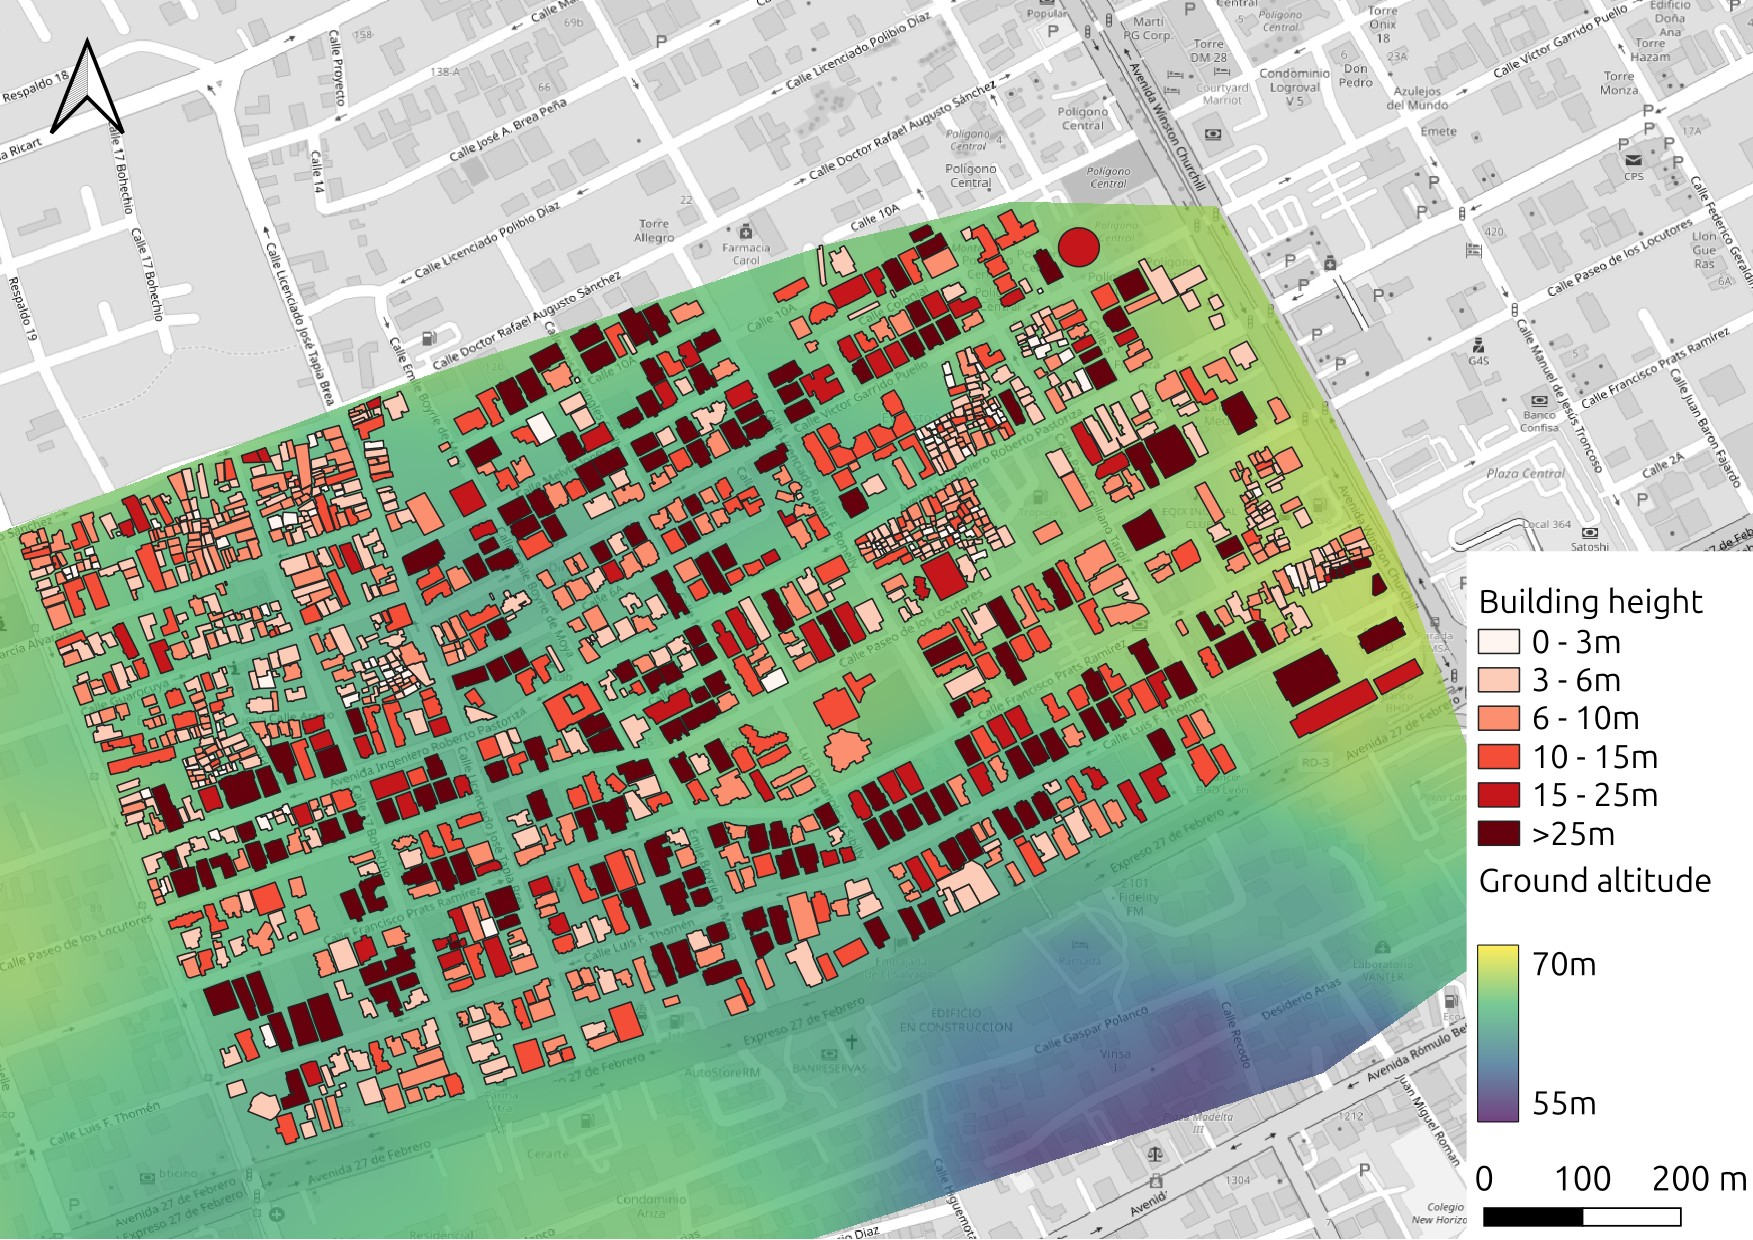
\includegraphics[width=\linewidth]{figures/santo_domingo_drone_height.jpg}
            \caption{Drone obtained building height}
            \label{fig:drone_height}
        \end{subfigure} & 
        \begin{subfigure}[t]{0.45\linewidth}
            \centering
            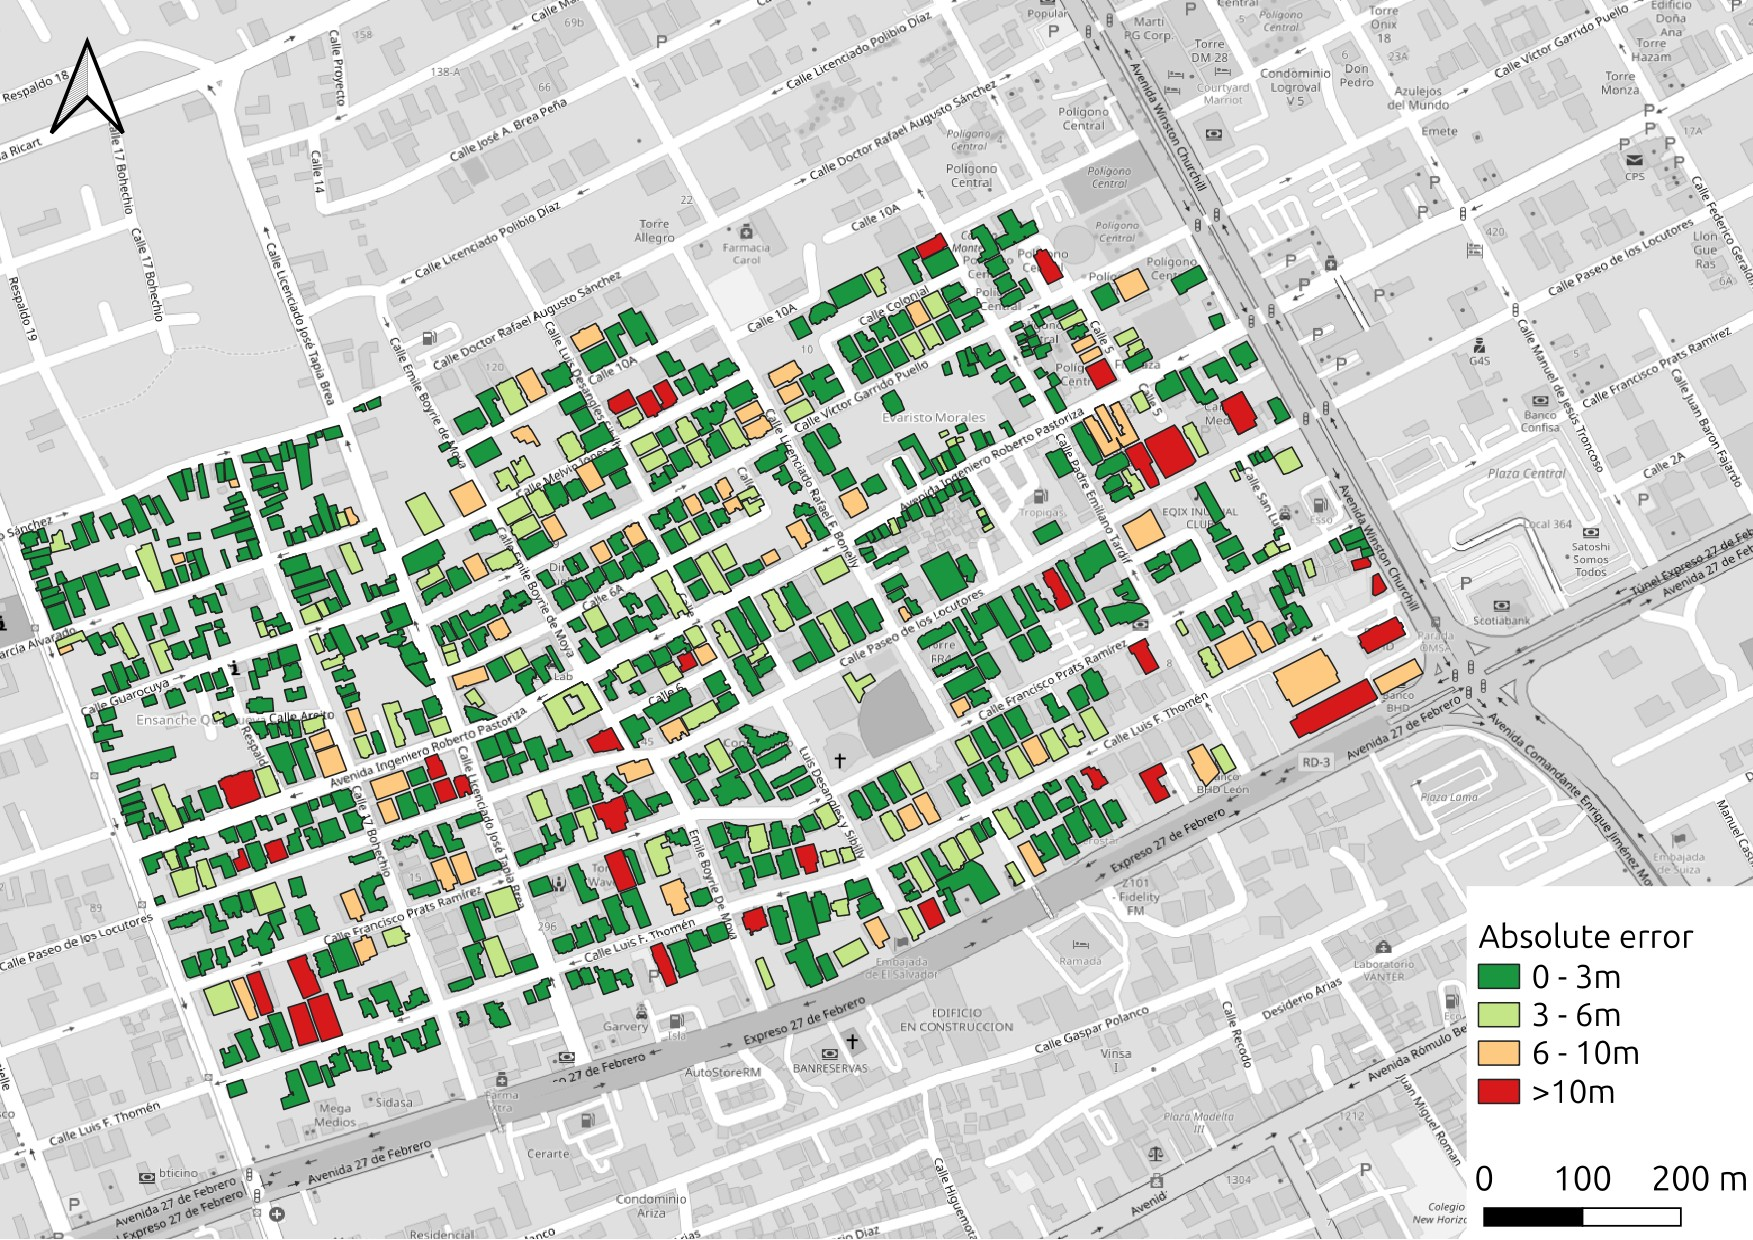
\includegraphics[width=\linewidth]{figures/santo_domingo_absolute_error.jpg}
            \caption{Absolute error (survey and drone)}
            \label{fig:abs_error}
        \end{subfigure}
    \end{tabular}
    \caption{Building heights obtained from a drone survey in the pilot region of Santo Domingo (Dominican Republic), along with the absolute error compared to field survey data on the number of floors (assuming 3 meters per floor).}
    \label{fig:height_results}
\end{figure}

\FloatBarrier

\renewcommand{\sectionnametext}{Construction year and building code quality}
\renewcommand{\headingtextR}{\thesection. \sectionnametext}
\section{\sectionnametext}

The results for building code quality are very constant in every pilot area as every neighbourhood was build around the same year (fig. \ref{fig:ductility_results}). The construction year has been obtained processing the World Settlement Footprint layer \footcite{marconcini_outlining_2020, marconcini_understanding_2021}. Instead of recording construction year building code quality allows for comparisons between buildings from different countries.

\begin{figure}[htbp]
    \centering
    \begin{tabular}{ccc}
        \begin{subfigure}[t]{0.3\linewidth}
            \centering
            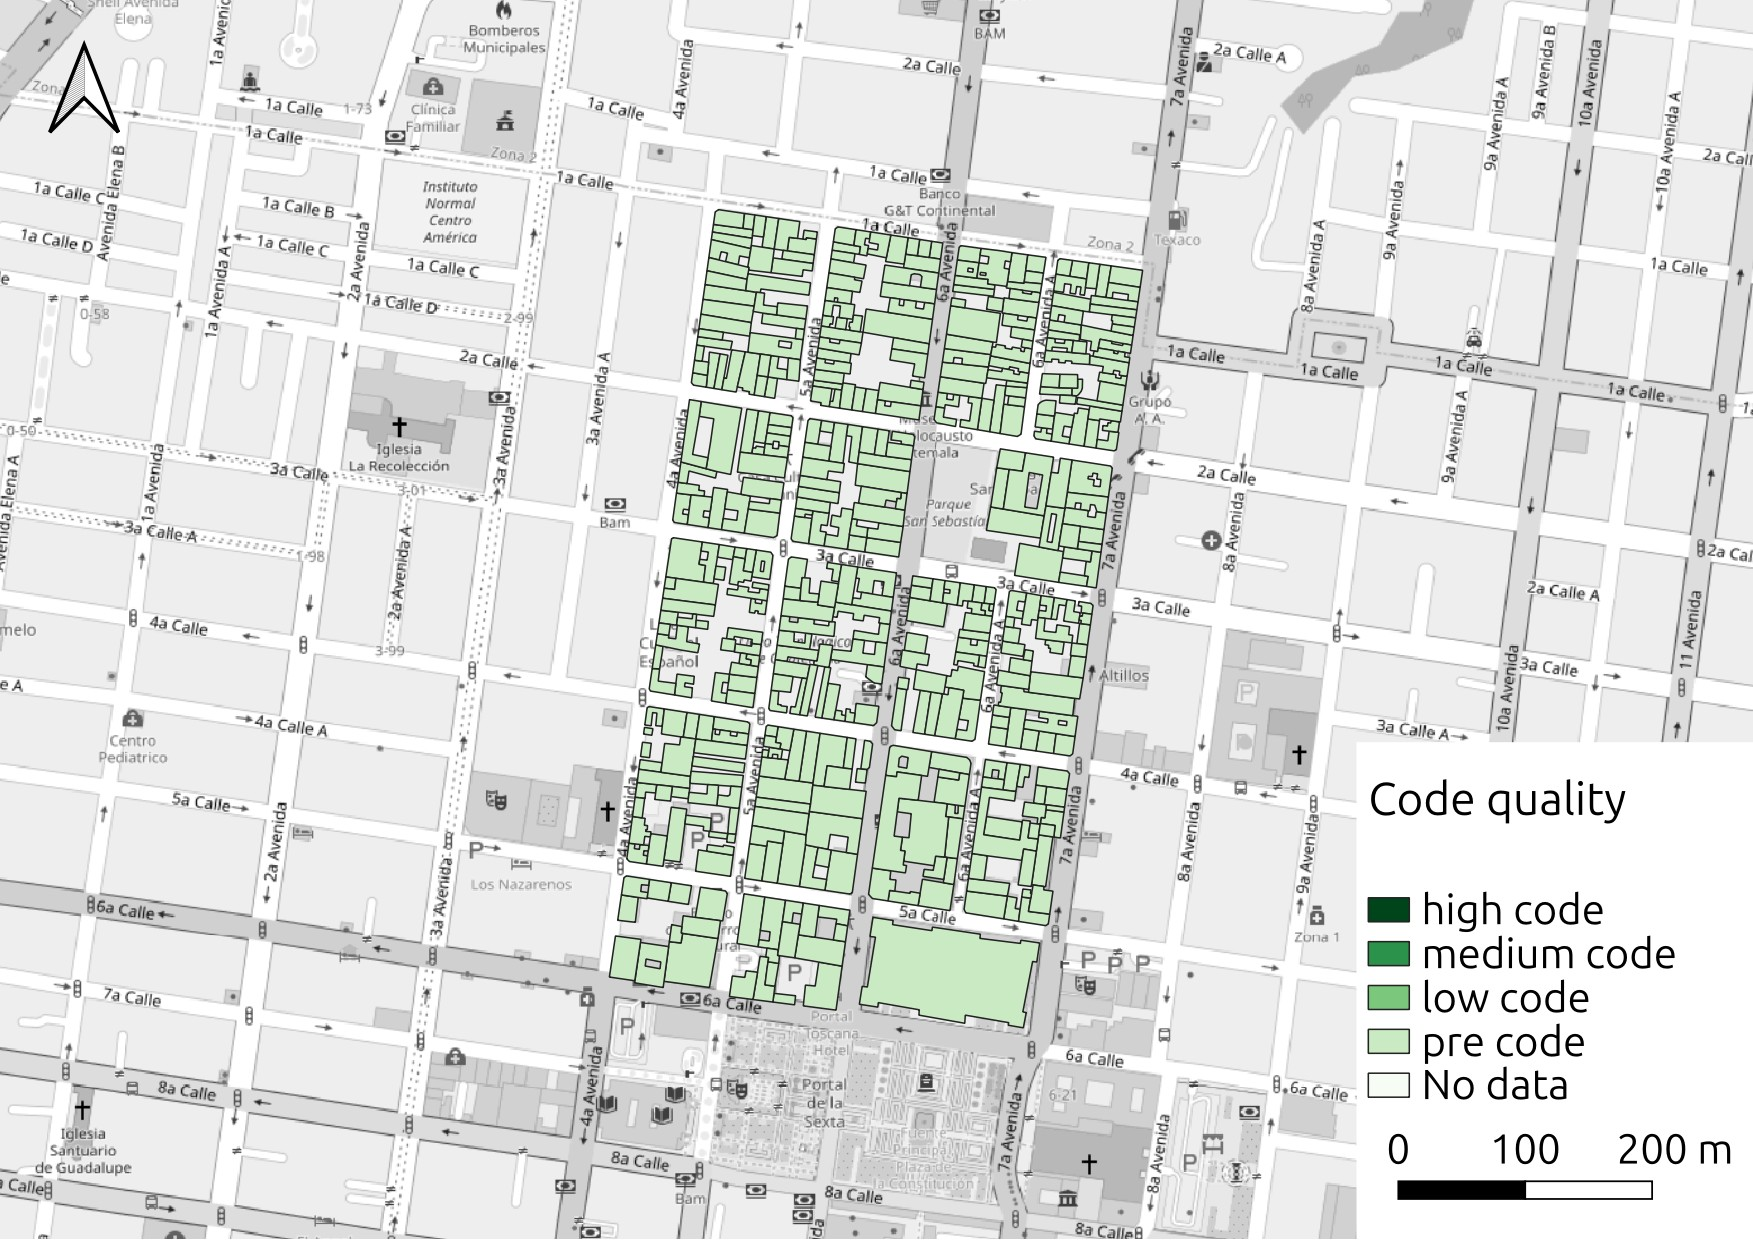
\includegraphics[width=\linewidth]{figures/year_Guatemala.jpg}
            \caption{Ciudad de Guatemala (Guatemala)}
        \end{subfigure} & 
        \begin{subfigure}[t]{0.3\linewidth}
            \centering
            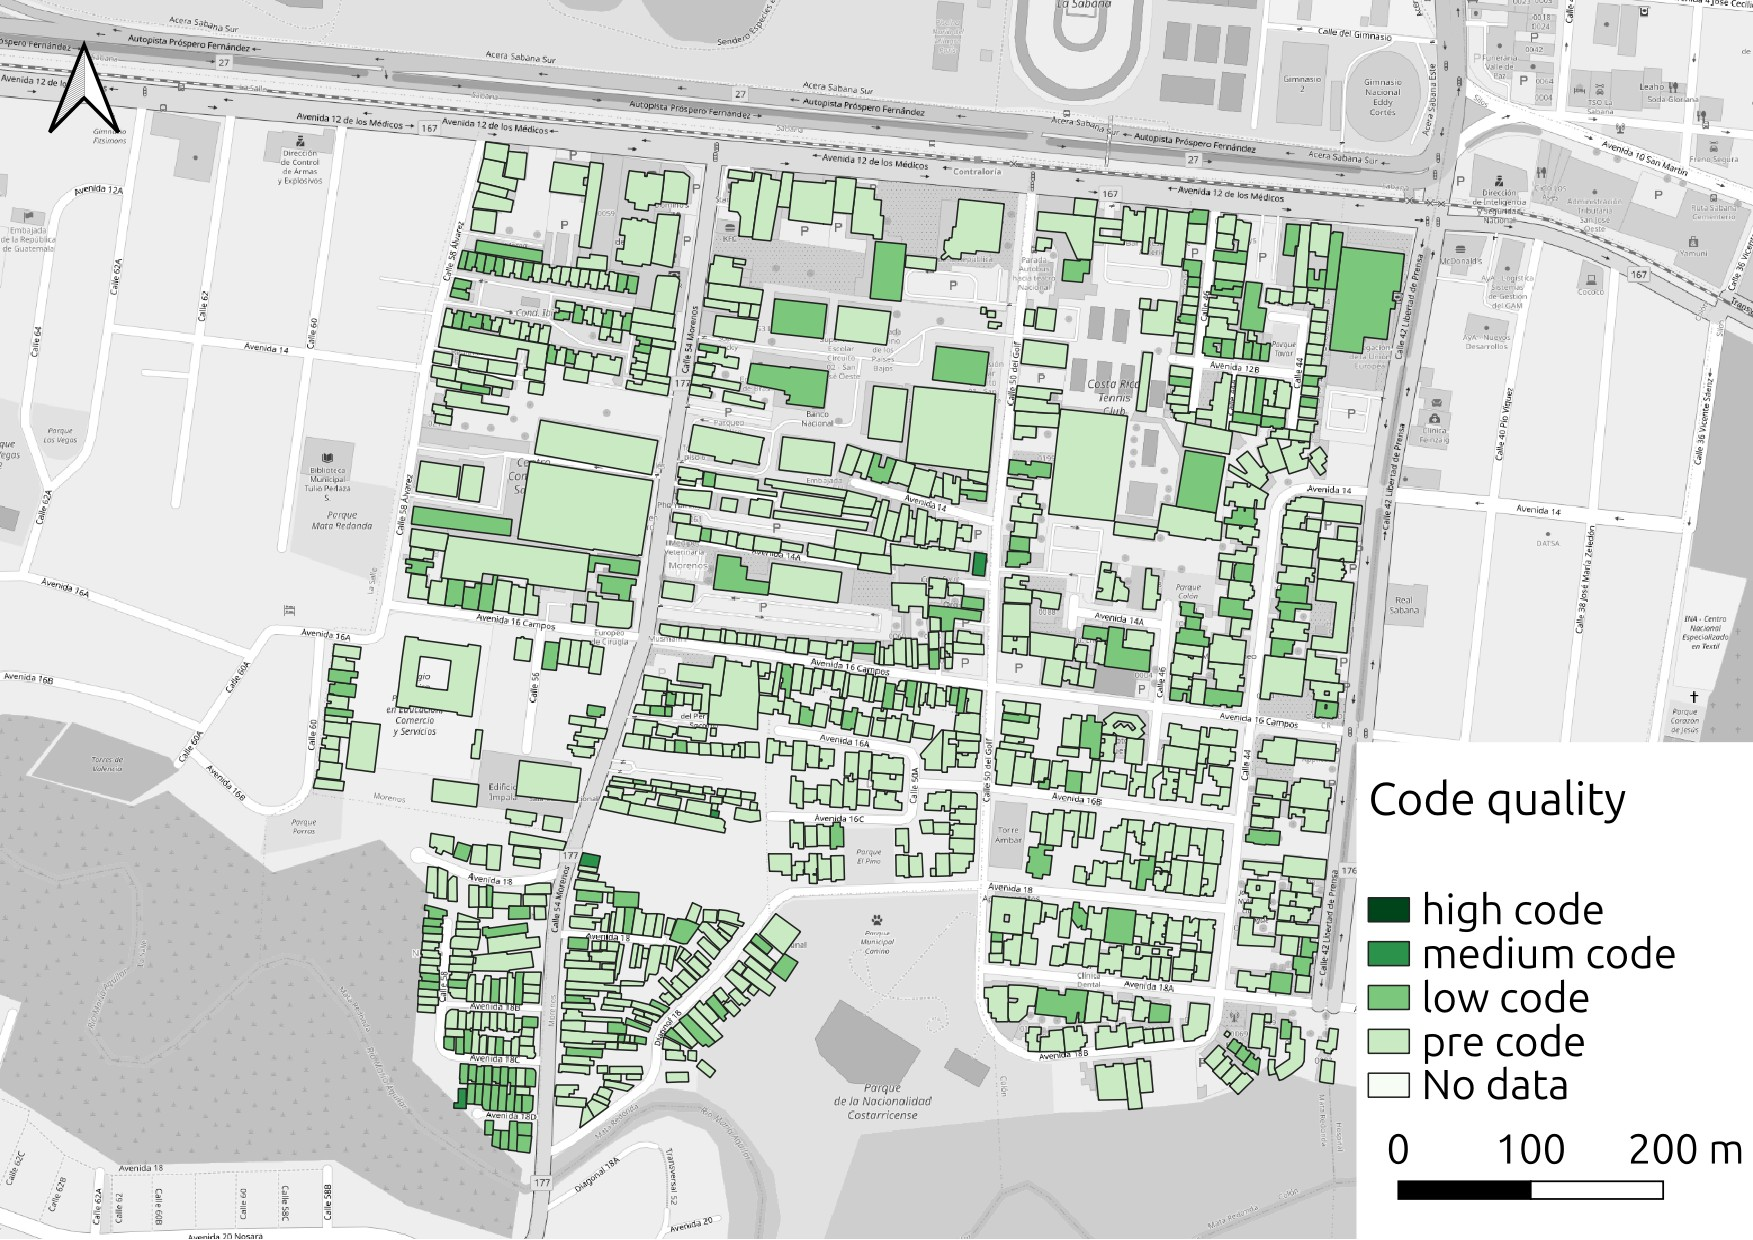
\includegraphics[width=\linewidth]{figures/year_San José.jpg}
            \caption{San Jośe (Costa Rica)}
        \end{subfigure}  & 
        \begin{subfigure}[t]{0.3\linewidth}
            \centering
            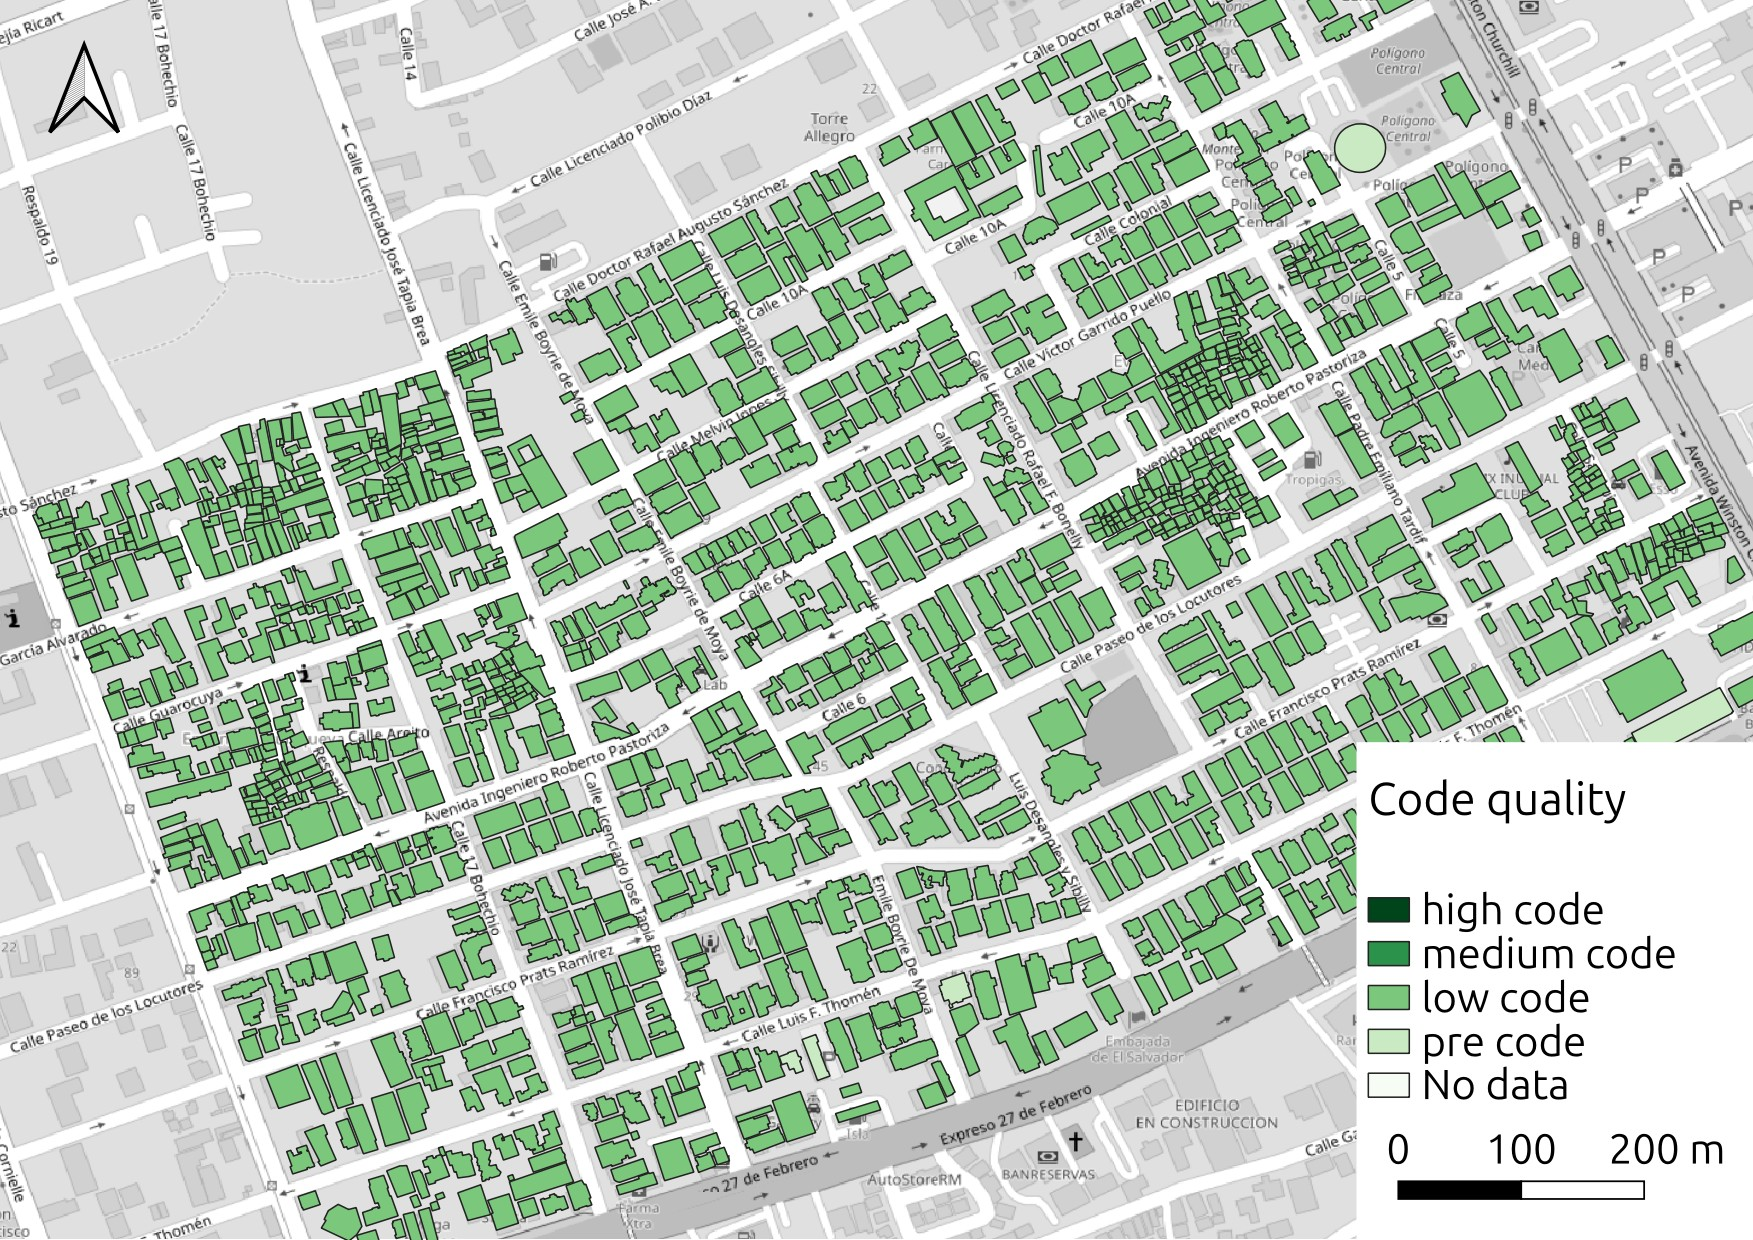
\includegraphics[width=\linewidth]{figures/year_Santo Domingo.jpg}
            \caption{Santo Domingo (Dominican Republic)}
        \end{subfigure} 
    \end{tabular}
    \caption{Building code type according to table \ref{tab:ductility_year}.}
    \label{fig:ductility_results}
\end{figure}

\FloatBarrier
\renewcommand{\sectionnametext}{Roof material}
\renewcommand{\headingtextL}{\shortchapternametext}
\renewcommand{\headingtextR}{\thesection. \sectionnametext}
\section{\sectionnametext}

The roof material results are shown in figure \ref{fig:roof_material_results}. The best results are obtained for an unsupervised classification of 4 classes divided in the following categories: bright and concrete roofs, dark and shadows, metallic materials and asphalt materials, usually concrete roof with asphalt covering for imperviousness. 

\begin{figure}[htbp]
    \centering
    \begin{tabular}{ccc}
        \begin{subfigure}[t]{0.3\linewidth}
            \centering
            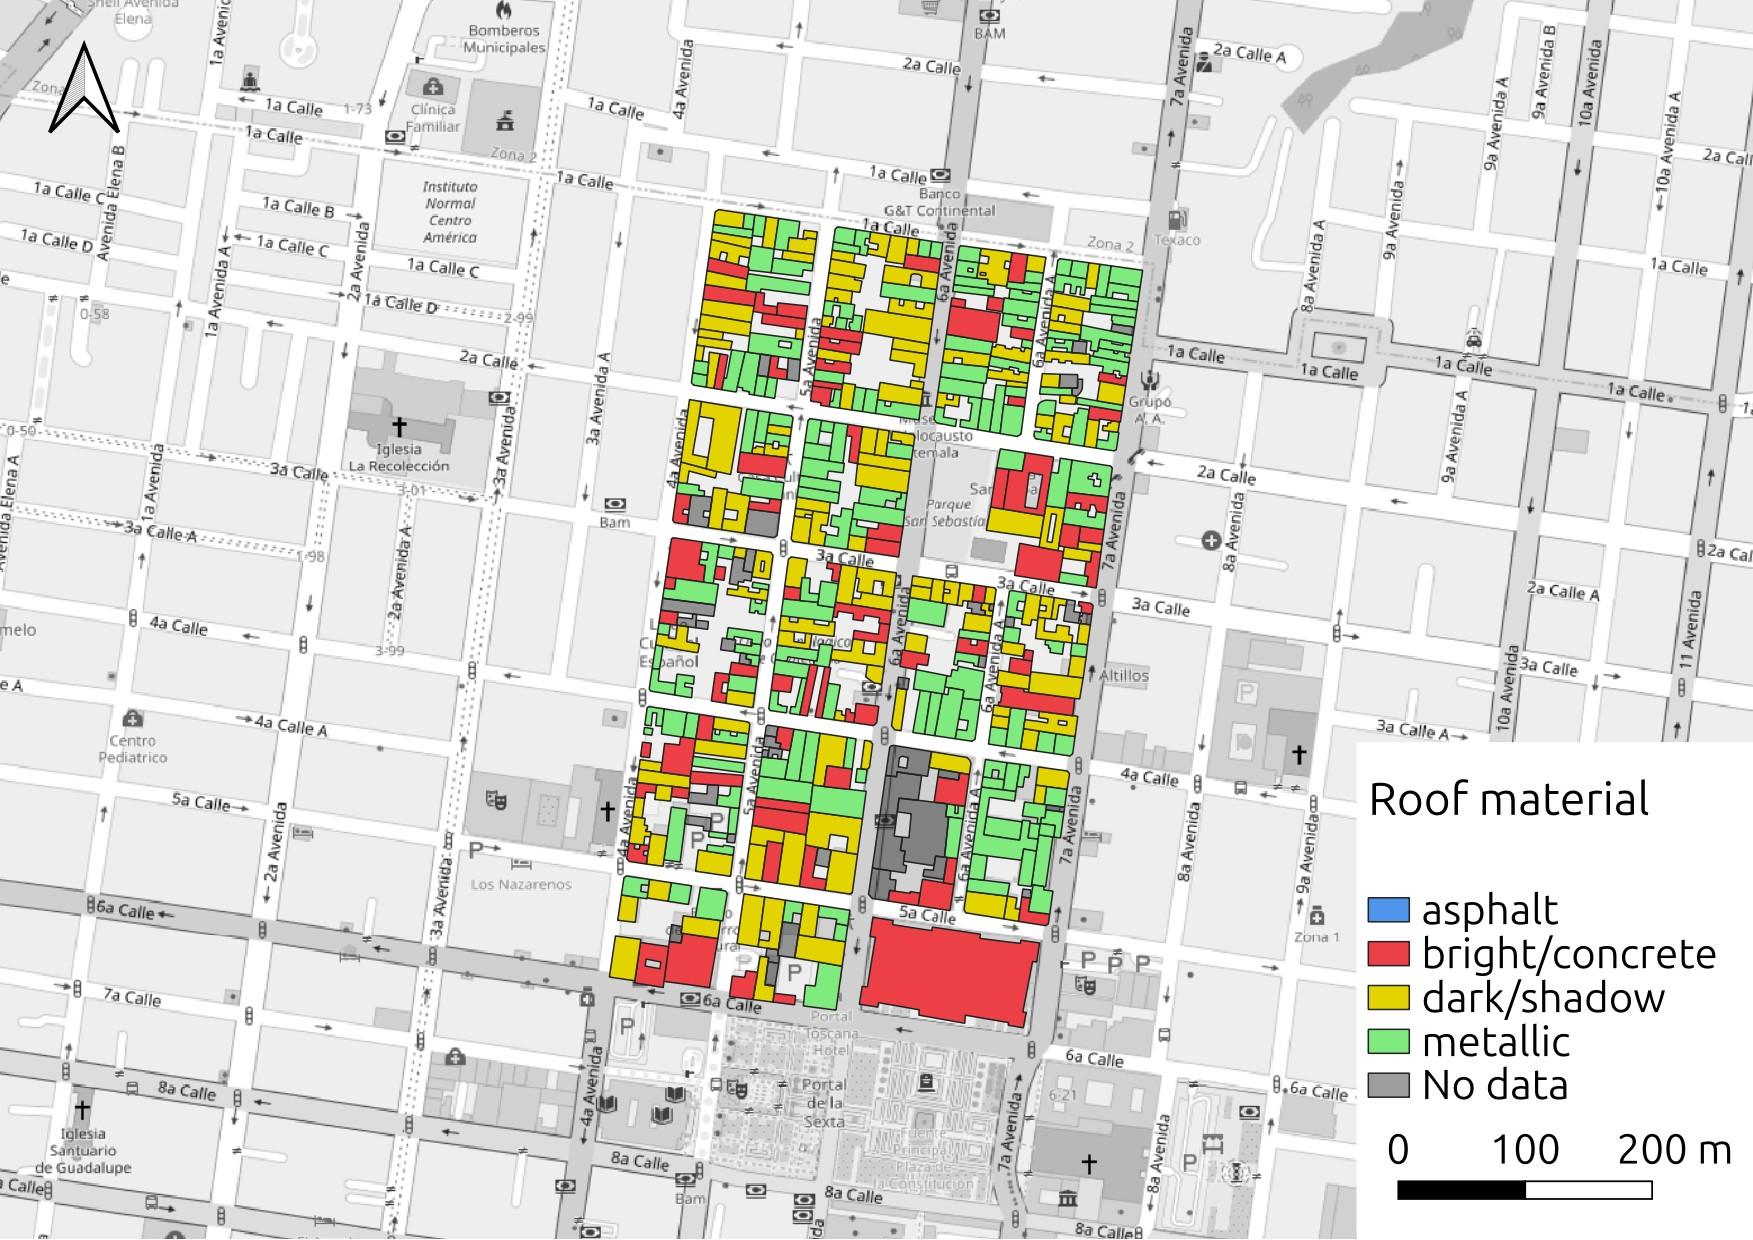
\includegraphics[width=\linewidth]{figures/roof_Guatemala.jpg}
            \caption{Ciudad de Guatemala (Guatemala)}
        \end{subfigure} & 
        \begin{subfigure}[t]{0.3\linewidth}
            \centering
            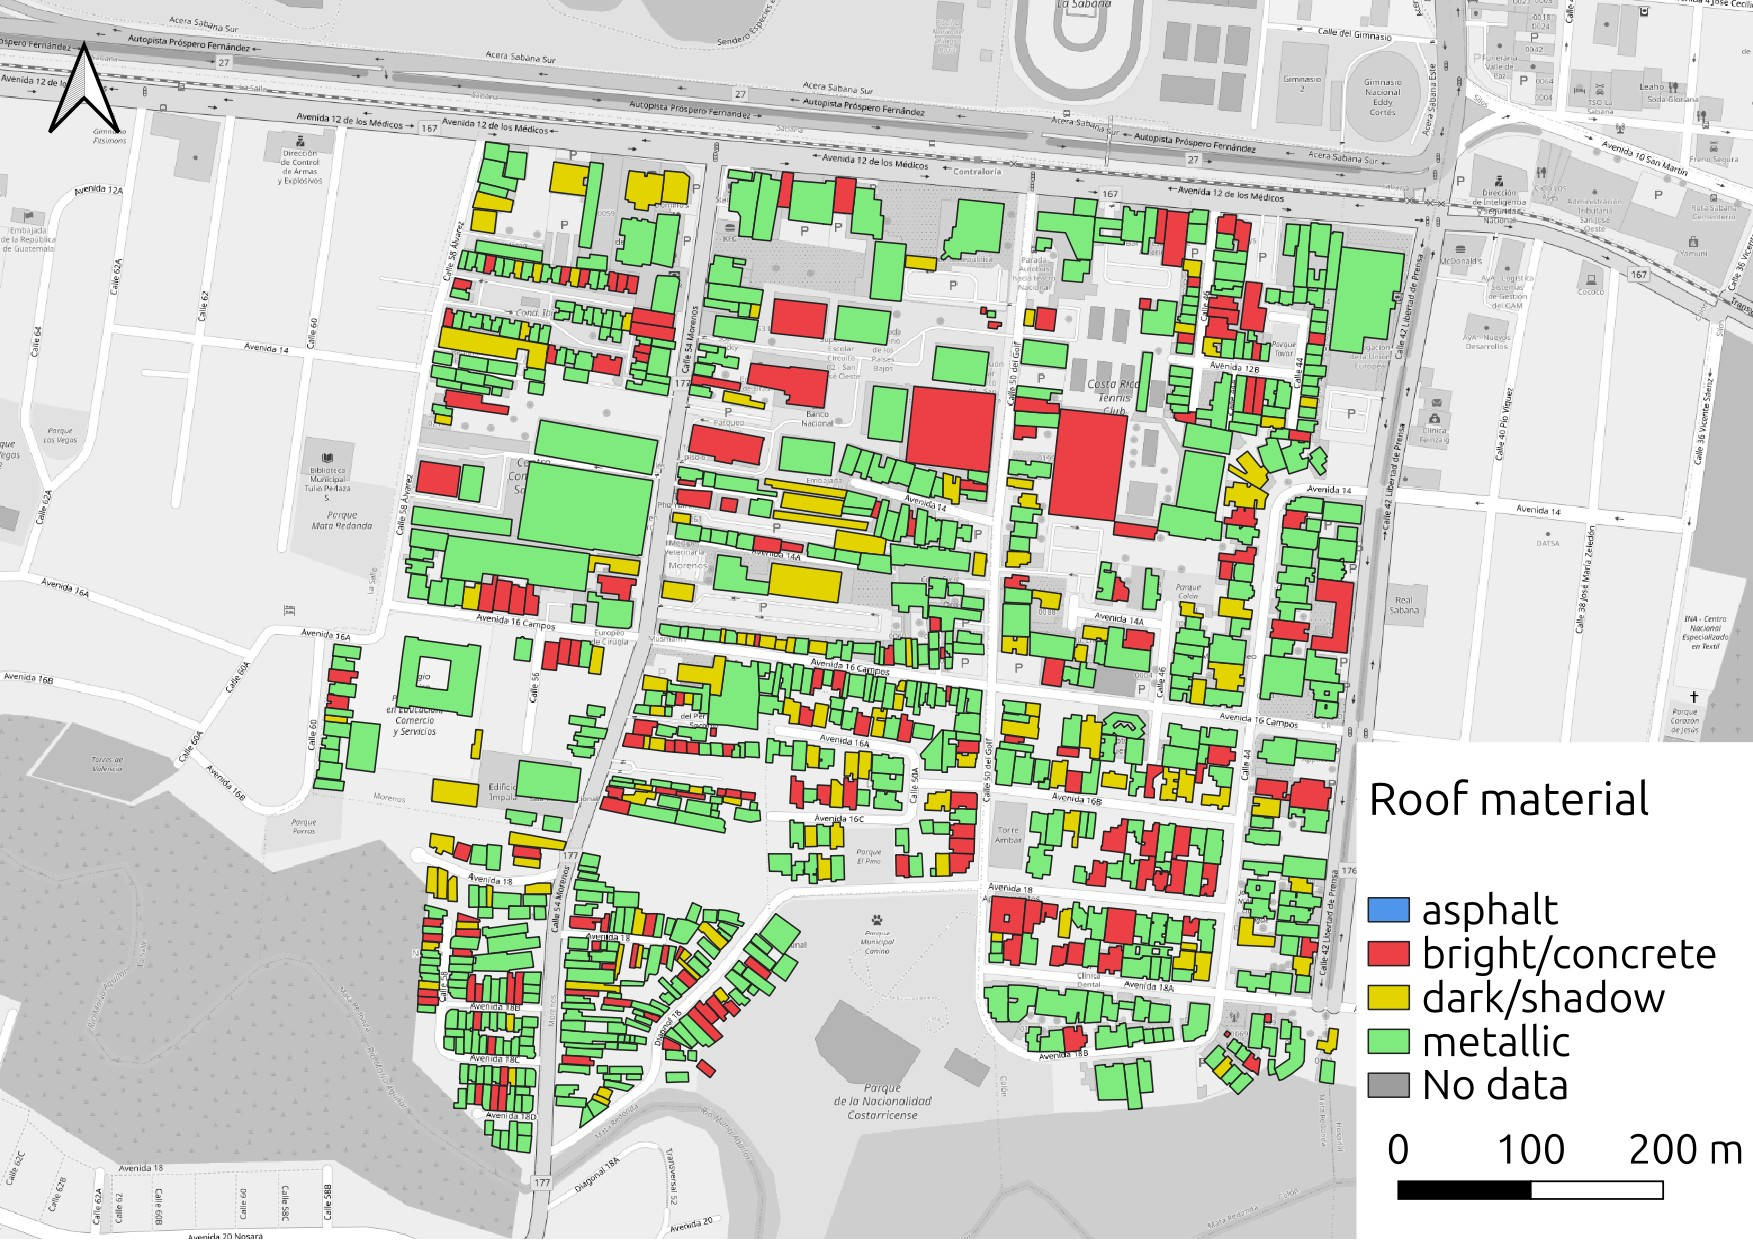
\includegraphics[width=\linewidth]{figures/roof_San José.jpg}
            \caption{San Jośe (Costa Rica)}
        \end{subfigure}  & 
        \begin{subfigure}[t]{0.3\linewidth}
            \centering
            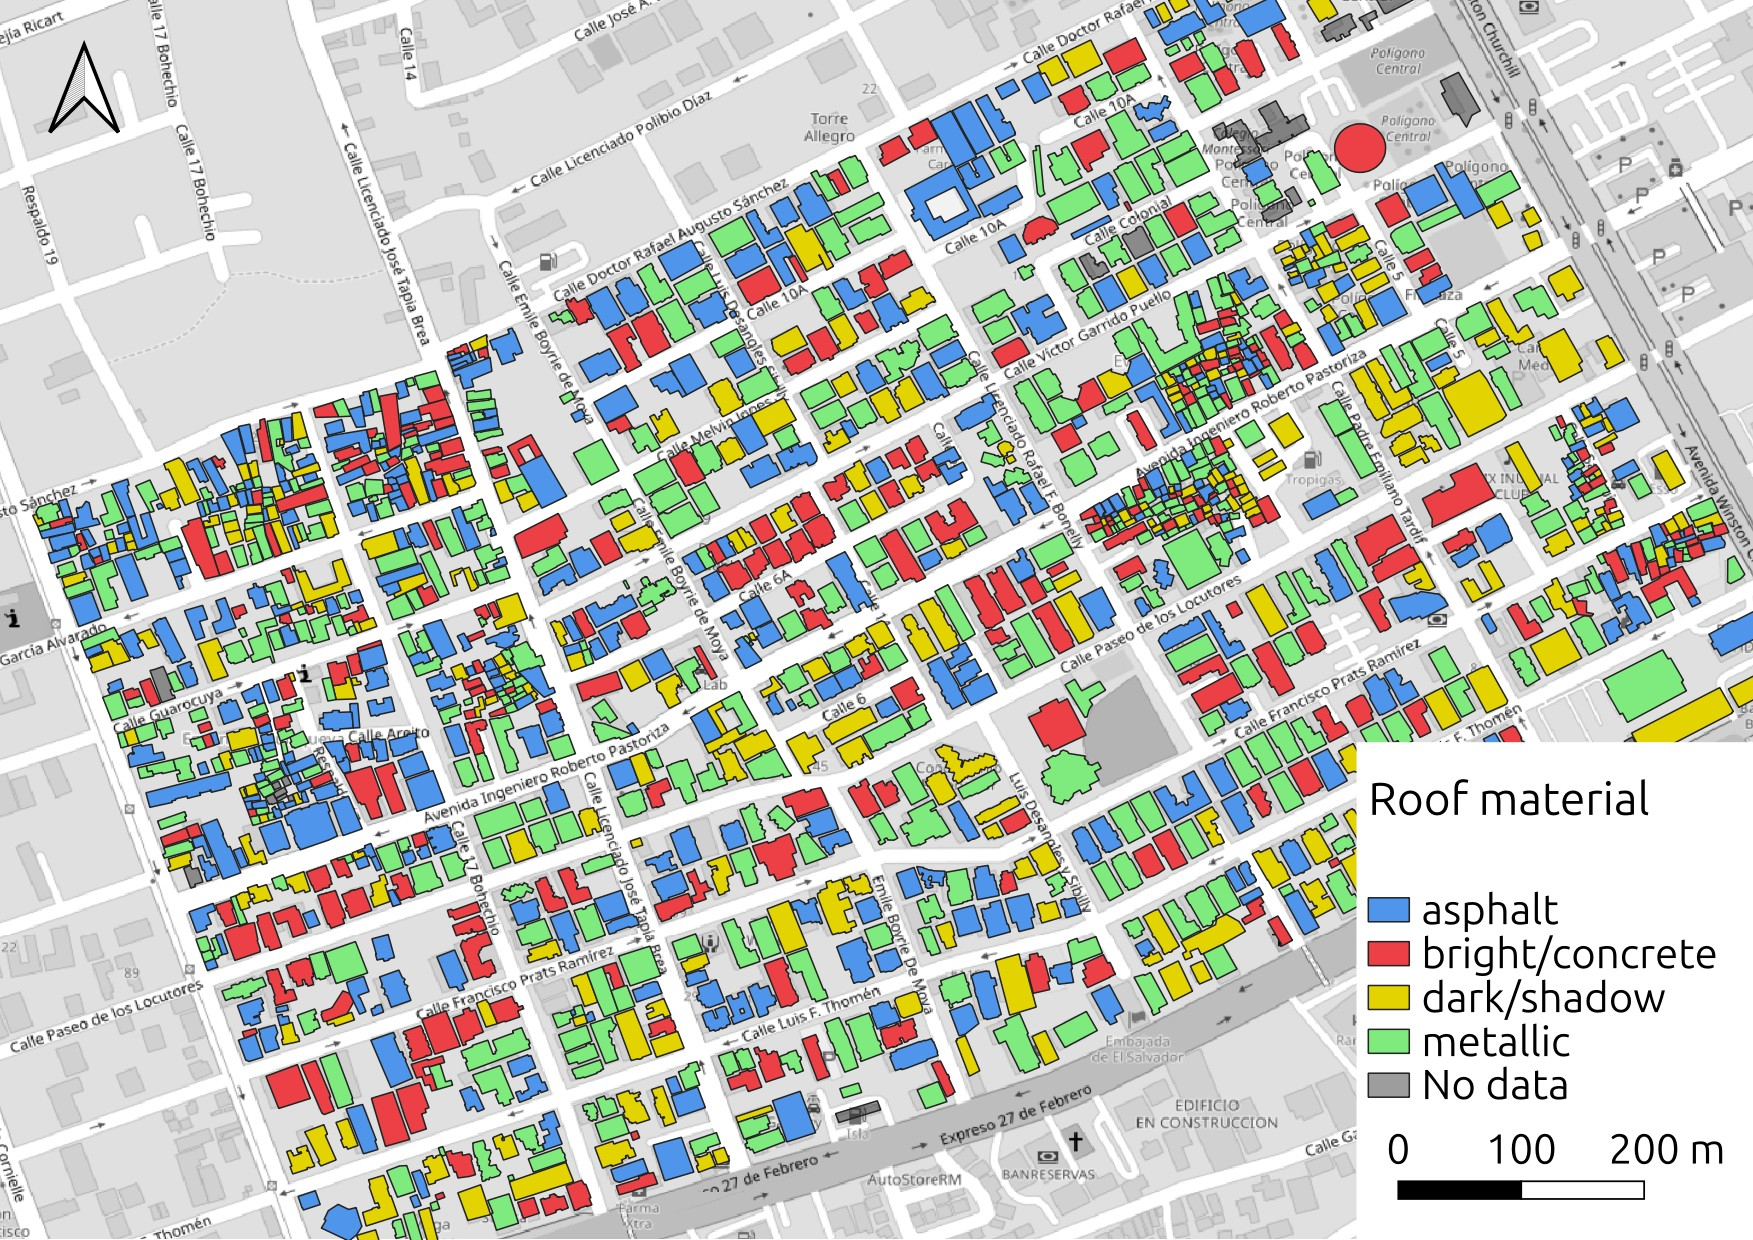
\includegraphics[width=\linewidth]{figures/roof_Santo Domingo.jpg}
            \caption{Santo Domingo (Dominican Republic)}
        \end{subfigure} 
    \end{tabular}
    \caption{Results for the roof material obtained with spectral satellite imagery in the three pilot regions.}
    \label{fig:roof_material_results}
\end{figure}


\newpage

\renewcommand{\sectionnametext}{References}
\renewcommand{\headingtextR}{\thesection. \sectionnametext}
\section{\sectionnametext}
\printbibliography[heading=none]

\end{refsection}